\documentclass[12pt,a4paper]{extarticle}
\usepackage[utf8]{ inputenc }
\usepackage[russian]{ babel }
\usepackage[left=2.0cm, top=1.5cm, right=2.0cm, bottom=2.5cm]{ geometry }
\usepackage{ indentfirst }
\sloppy
\usepackage{ amsmath }
\usepackage{ amsfonts }
\usepackage{ amssymb }
\usepackage{ graphicx }
\usepackage{ subfig }
\usepackage{ gensymb }
\usepackage{ multicol } 
\usepackage{ cite }
\newcommand{\numofcol}{6}
\graphicspath{{images/}}

\begin{document}

\begin{center}
\textbf{\textsc{Построение средних спектров пятен микроволнового излучения по данным карты миссии Planck}}\\
Отчет по научно--исследовательской практике студента Пушкарева~В.В., 2018
Руководитель: Верходанов~О.В.
\vskip10pt
\hrule
\vskip20pt
\end{center}

В рамках научно--исследовательской практики в июле 2018 года проведено построение средних спектров пятен микроволнового фонового излучения по данным карт миссии Планк (версия 2015 года) для большой выборки пятен. Важность задачи объясняется тем, что при исследовании спектров отдельных пятен, выделяемых на карте реликтового излучения SMICA мисии Planck, было замечено, что часть таких спектров не имеет форму чернотельного типа, которая должна наблюдаться для пятен, связанных с флуктуациями температуры реликтового излучения. Для выяснения статистической значимости этого эффекта Верходановым~О.В. было предложено рассмотреть достаточно большую выборку пятен (порядка 1000), для которой построить усредненные спектры. Отдельный интерес при этом представляло исследование зависимости среднего спектра от углового размера сглаживания карты.

Решение задачи проводилось следующими основными шагами:
\begin{enumerate}
\item знакомство с литературой и основными инструментами анализа микроволнового излучения;
\item выбор площадок на картах микроволнового фона разных частот (30 MHz --- 217 MHz);
\item построение калибровки перевода интегральных интенсивностей в плотности потока по данным каталога радиоисточников Planck для карт разных частот и разных угловых размеров сглаживаний карты;
\item построение средних спектров пятен микроволнового фона с измерением амплитуды пятен;
\item построение калиброванных средних спектров пятен микроволнового фона с измерение плотности потока.
\end{enumerate} 
Для выполнения последних трех пунктов написан ряд скриптов, использующих существующие пакеты программ для анализа карт микроволнового излучения.

\section{Предварительная подготовка}
На первом шаге проведено внимательное чтение статей, понимание результатов и методов которых необходимо для решения поставленной задачи. Это исчерпывающий обзор~\cite{overview_Verkhodanov:2016}, описание схемы GLESP --- ~\cite{GLESP:2005} и статья~\cite{Verkhodanov_etal:2015}, где проведена калибровка перевода интегральных интенсивностей в плотности потока по данным каталога RCR (такую же калибровку, но только по источникам из каталога Planck необходимо было повторить и в данной задаче). Важным подготовительным этапом было также знакомство с существующими инструментами, применимыми для эффективного анализа микроволнового излучения и визуализации результатов, --- пакетом программ \texttt{GLESP}, \texttt{SExtractor}, \texttt{Gnuplot}, а также элементами скриптовых языков программирования \texttt{BASH} и \texttt{Python}. 

\section{Выбор площадок}
На картах микроволнового фона было выбрано 19 прямоугольных площадок размером $20\degree \times 20\degree$ в таких областях, где вклад микроволнового излучения, связанного с Галактикой, во всём исследуемом диапазоне частот (30 MHz --- 217 MHz) является минимальным. Б\'{о}льшие частоты (353, 417 и 817 MHz) не анализировались, потому что этот вклад становится слишком большим. Расположение выбранных площадок показано на рисунке~\ref{big_areas}.
	\begin{figure}[h!]
		\begin{center}
			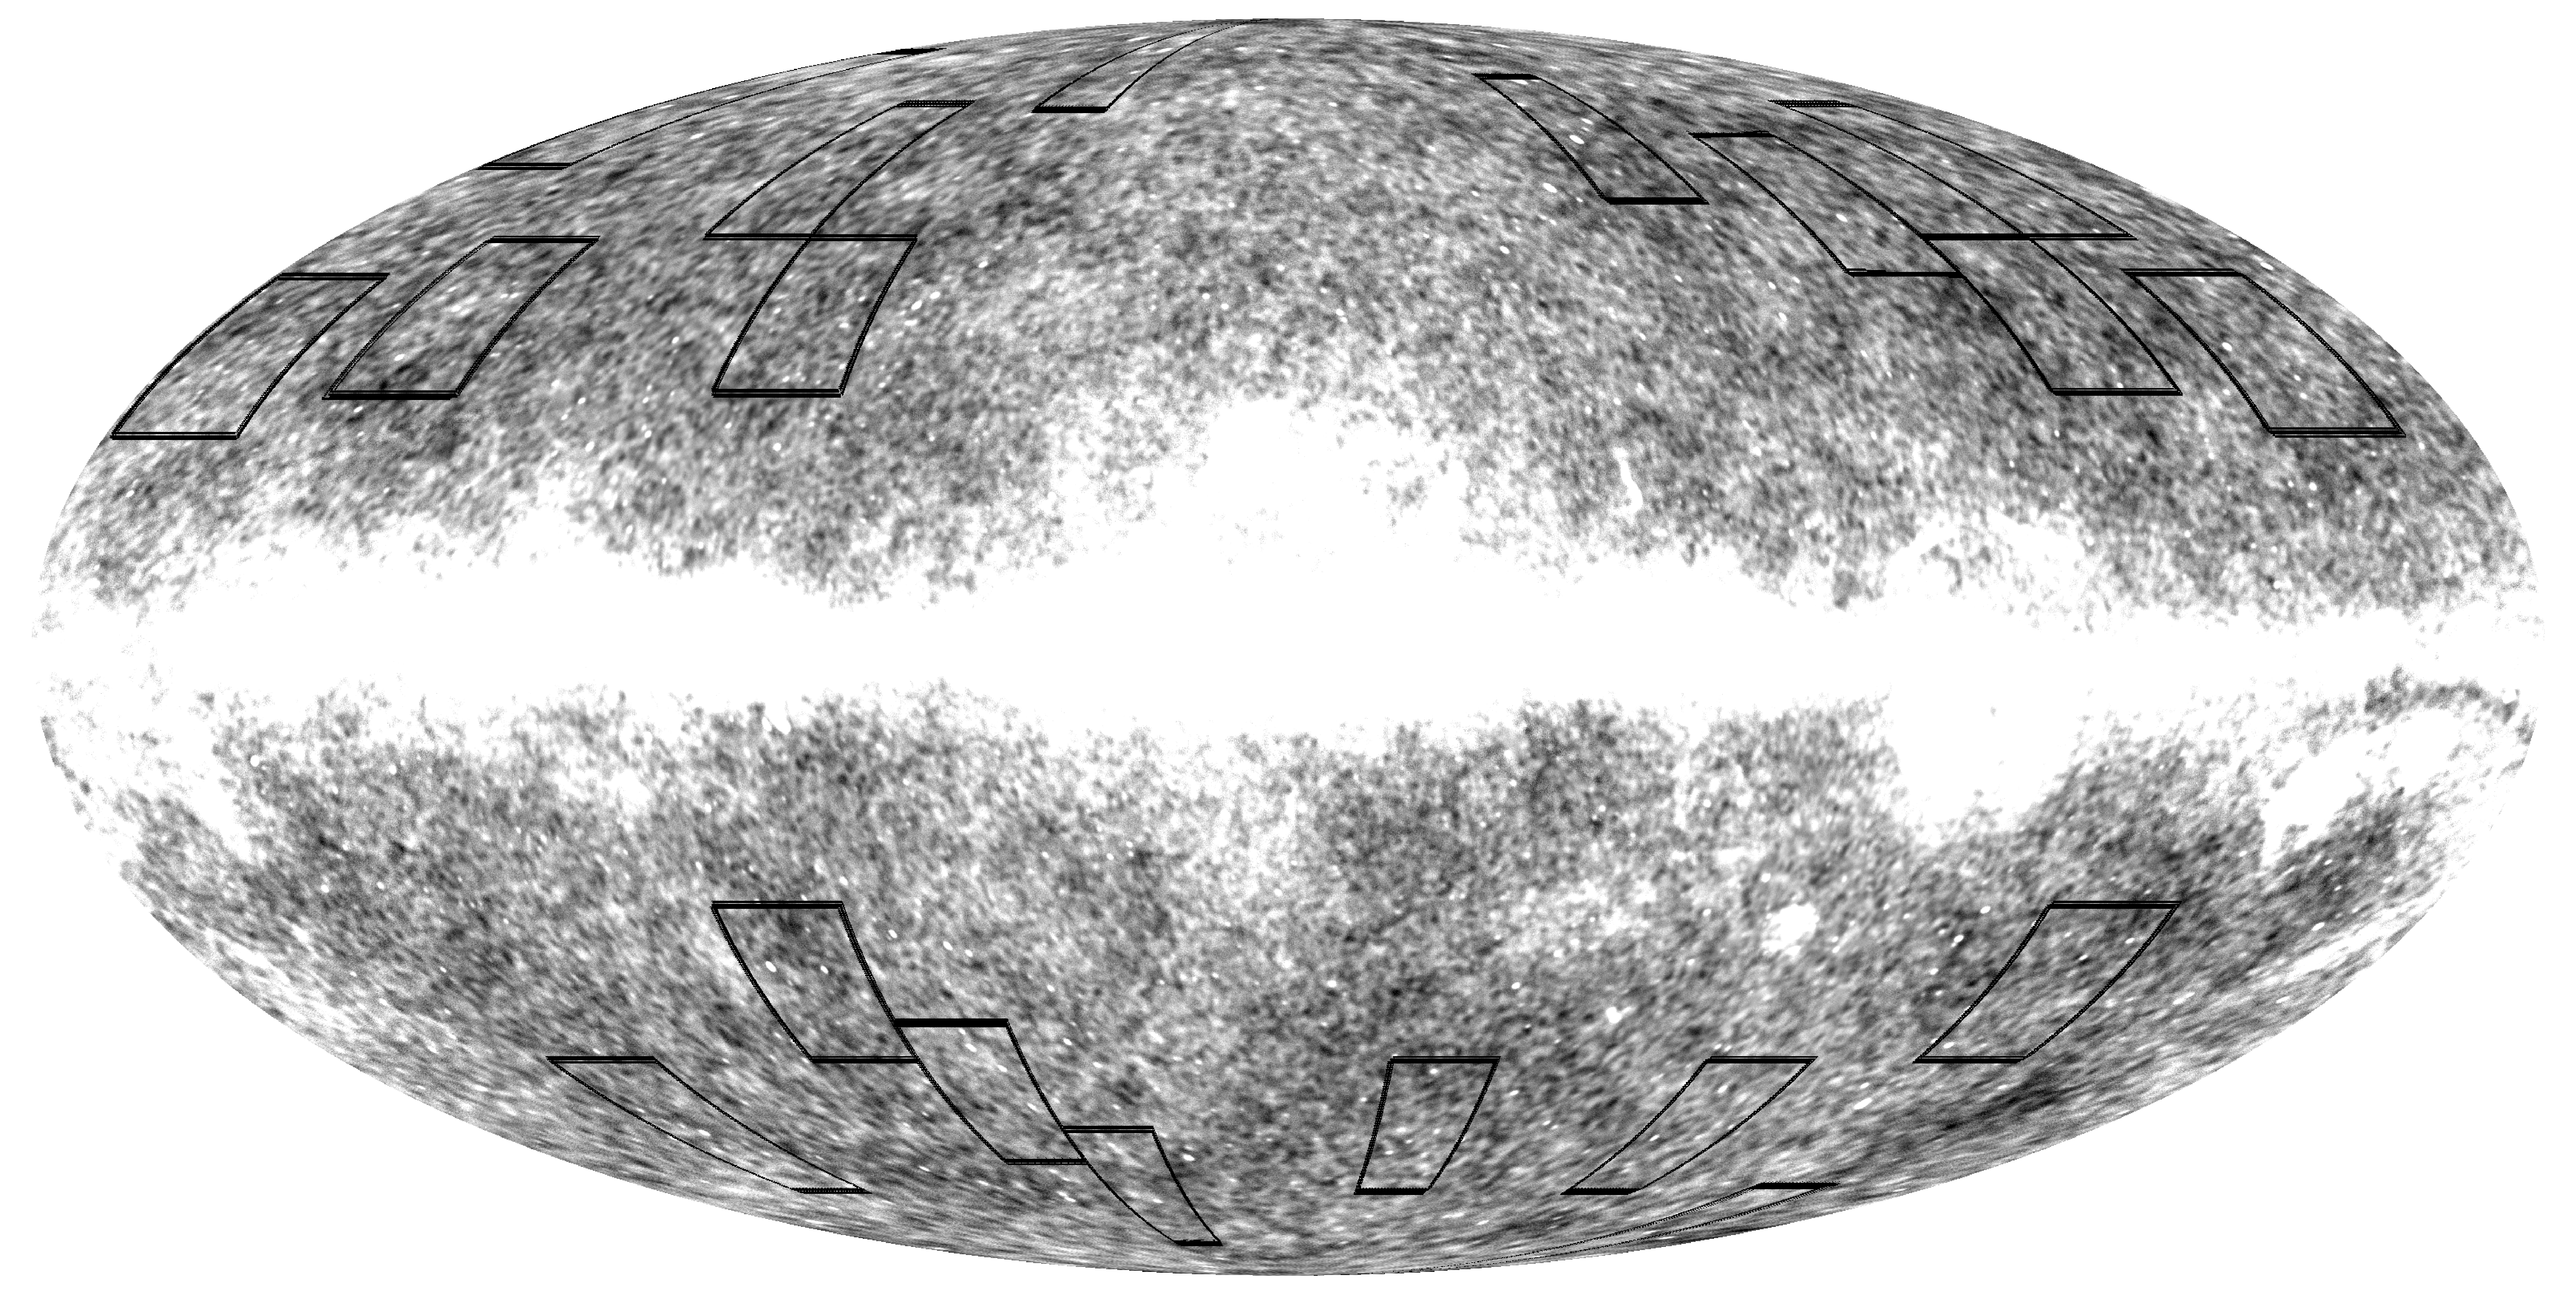
\includegraphics[width=0.8\textwidth]{areas_030_wb}
			\caption{Расположение площадок размером $20\degree \times 20\degree$ на карте частотой 30 MHz}
			\label{big_areas}
		\end{center}
	\end{figure}

\section{Калибровка}
На картах микроволнового излучения, подготовленных миссией Planck, интенсивность излучения характеризуется температурой в градусах по шкале Кельвина. Однако в радиоастрономии общепринятой шкалой являются плотности потока в Янских. Нами была проведена калибровка перевода интегральных интенсивностей, измеренных с помощью программы \texttt{SExtractor}, в плотности потока. Данная процедура была проведена для карт всех исследуемых частот и различных угловых размеров сглаживания (0, 5, 35, 60 arcmin). Для построения калибровки из карты соответствующей частоты и соответствующего сглаживания вырезались квадратные области размером полторы диаграммы направленности, координаты центров которых соответствовали координатам источника в каталоге Planck. Вырезанные области затем подавались на вход программы \texttt{SExtractor}. На рисунках~\ref{calib_0} и~\ref{calib_corr_030_conv} показаны примеры построенных калибровочных кривых. На рисунках~\ref{corr_0} и~\ref{calib_corr_030_conv} показаны также зависимости плотности потока для источников из каталога Planck от плотности потока, рассчитанной из интегральной интенсивности, позволяющие оценить правдоподобность построенной калибровки. Результаты калибровки приведены в таблице~\ref{tab:calib}.
	\begin{figure}[h!]
		\begin{tabular}{ccc}
			\subfloat[30 MHz $a=3.30$]{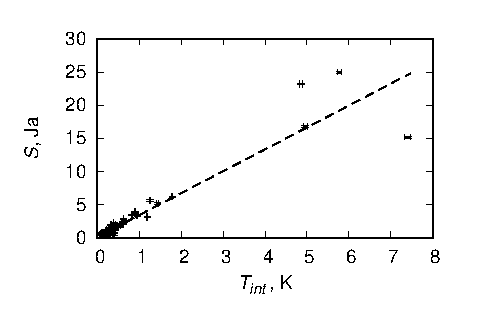
\includegraphics[width=0.33\textwidth]{030_0_wb}} &
			\subfloat[44 MHz $a=4.72$]{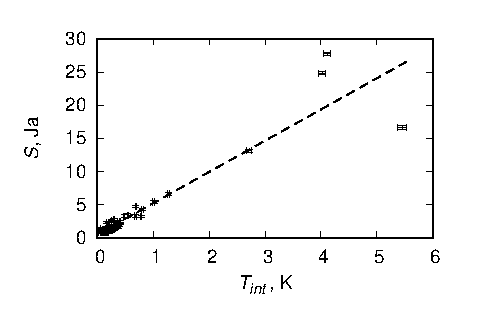
\includegraphics[width=0.33\textwidth]{044_0_wb}} &
			\subfloat[70 MHz $a=12.4$]{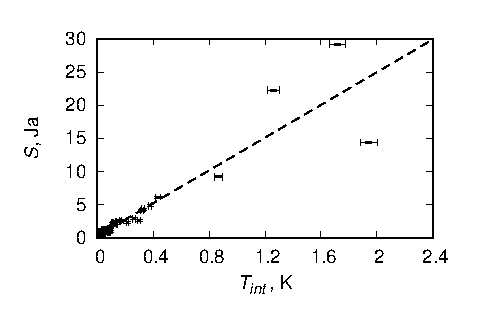
\includegraphics[width=0.33\textwidth]{070_0_wb}} \\
			\subfloat[100 MHz $a=20.6$]{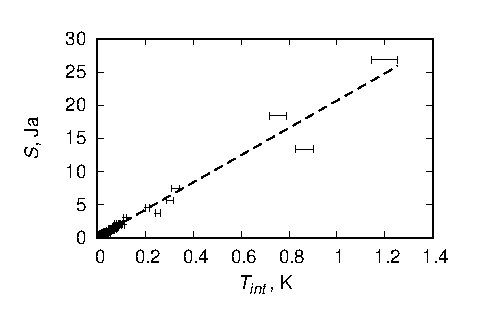
\includegraphics[width=0.33\textwidth]{100_0_wb}} &
			\subfloat[143 MHz $a=30.6$]{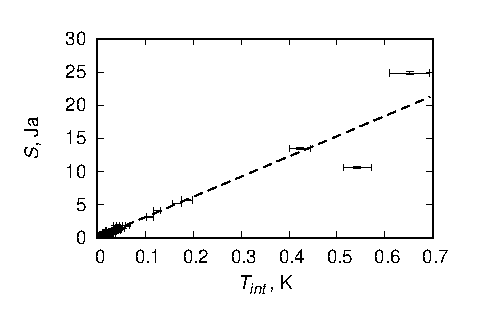
\includegraphics[width=0.33\textwidth]{143_0_wb}} &
			\subfloat[217 MHz $a=35.7$]{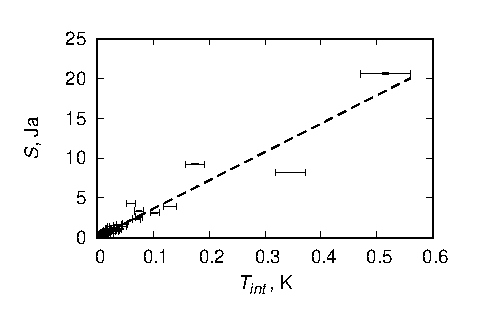
\includegraphics[width=0.33\textwidth]{217_0_wb}} 
		\end{tabular}
		\caption{Зависимости плотности потока для источников из каталога Planck от интегральной интенсивности, измеренной по картам микроволного излучения миссии Planck изофото-скорректированным методом, реализованным программой \texttt{SExtractor}, и калибровочные прямые; $a$ --- угловой коэффициент калибровочной прямой. Использована выборка порядка 100 источников}
		\label{calib_0}
	\end{figure}

	\begin{figure}[h!]
		\begin{tabular}{ccc}
			\subfloat[30 MHz]{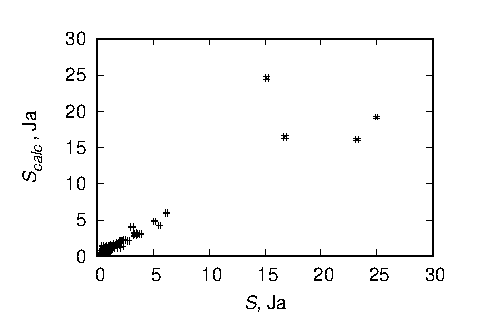
\includegraphics[width=0.33\textwidth]{corr_030_0_wb}} &
			\subfloat[44 MHz]{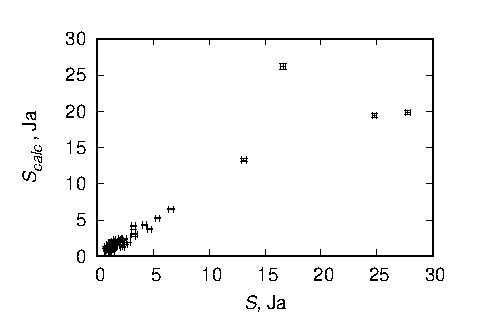
\includegraphics[width=0.33\textwidth]{corr_044_0_wb}} &
			\subfloat[70 MHz]{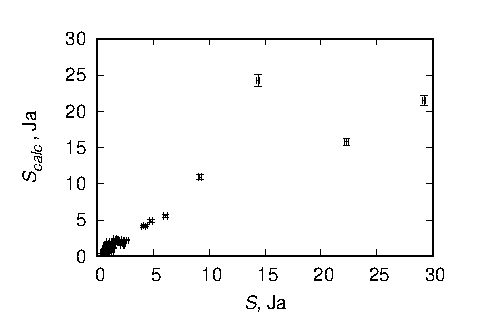
\includegraphics[width=0.33\textwidth]{corr_070_0_wb}} \\
			\subfloat[100 MHz]{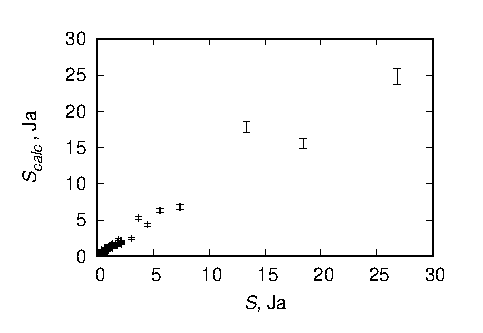
\includegraphics[width=0.33\textwidth]{corr_100_0_wb}} &
			\subfloat[143 MHz]{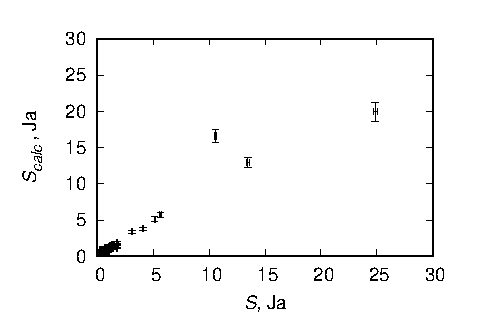
\includegraphics[width=0.33\textwidth]{corr_143_0_wb}} &
			\subfloat[217 MHz]{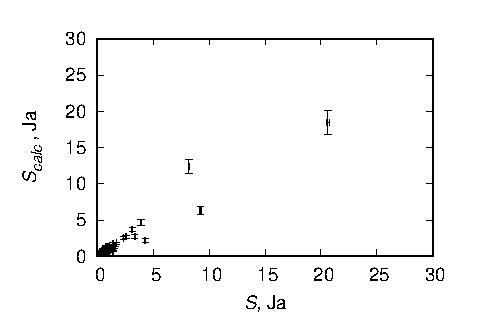
\includegraphics[width=0.33\textwidth]{corr_217_0_wb}} 
		\end{tabular}
		\caption{Зависимости плотности потока для источников из каталога Planck от плотности потока, рассчитанной из интегральной интенсивности, измеренной по картам микроволного излучения}
		\label{corr_0}
	\end{figure}

	\begin{figure}[h!]
		\begin{tabular}{ccc}
			\subfloat[30 MHz --- 5 arcmin \newline $a=3.21$]{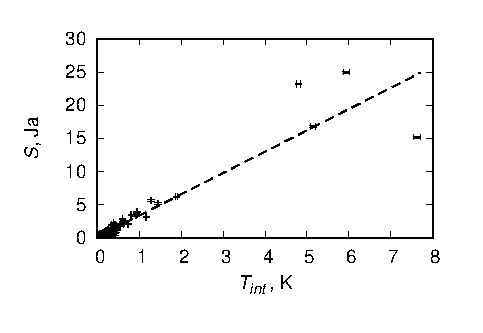
\includegraphics[width=0.33\textwidth]{030_5_wb}} &
			\subfloat[30 MHz --- 35 arcmin \newline $a=190$]{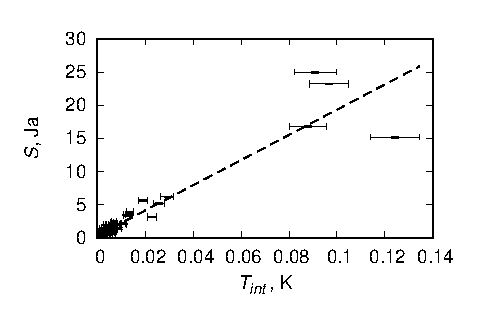
\includegraphics[width=0.33\textwidth]{030_35_wb}} &
			\subfloat[30 MHz --- 60 arcmin \newline $a=323$]{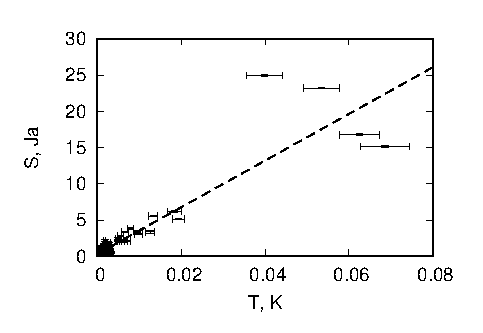
\includegraphics[width=0.33\textwidth]{030_60_wb}} \\
			\subfloat[30 MHz --- 5 arcmin]{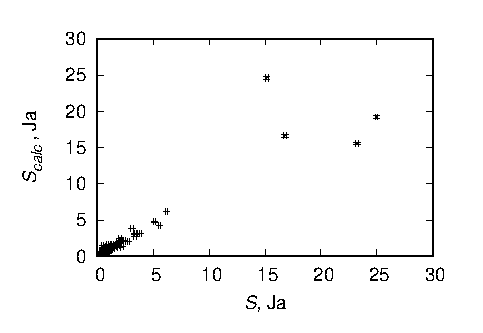
\includegraphics[width=0.33\textwidth]{corr_030_5_wb}} &
			\subfloat[30 MHz --- 35 arcmin]{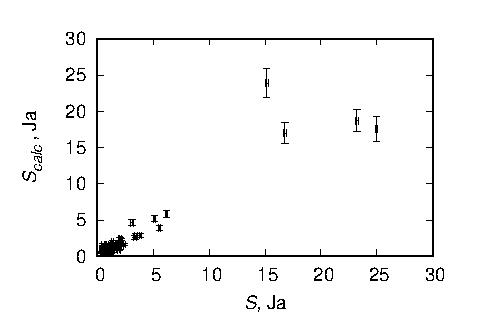
\includegraphics[width=0.33\textwidth]{corr_030_35_wb}} &
			\subfloat[30 MHz --- 60 arcmin]{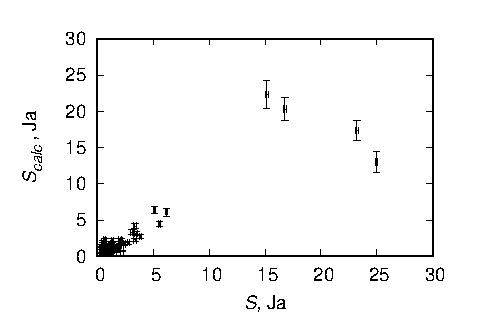
\includegraphics[width=0.33\textwidth]{corr_030_60_wb}} 
		\end{tabular}
		\caption{a, b, c: зависимости плотности потока на частоте $30$ MHz для источников из каталога Planck от интегральной интенсивности, измеренной по картам микроволного излучения для различных угловых размеров сглаживания карты; $a$ --- угловой коэффициент калибровочной прямой\\ d, e, f: зависимости плотности потока для источников из каталога Planck от плотности потока, рассчитанной из интегральной интенсивности, измеренной по сглаженным картам микроволнового излучения}
		\label{calib_corr_030_conv}
	\end{figure}

\begin{table}[h!]
	\setcaptionmargin{0mm}
	\caption{Параметры калибровочных кривых. Здесь $cr$ --- угловой размер сглаживания, $\sigma_a$ --- относительная ошибка определения углового коэффициента прямой, $N_s$ --- размер выборки источников из каталога}
	\label{tab:calib}
	\medskip
	\begin{tabular}{c|c|c|c|c}
		$f$, MHz & $cr$, arcmin & $S$, Jy & $\sigma_a$ & $N_s$\\[3 pt] \hline
		30 & 0 & $3.3093T+0.0897$ & 3\% & 200\\[3 pt]
		30 & 5 & $3.2165T+0.1090$ & 3\% & 200\\[3 pt]
		30 & 35 & $190.2627T+0.2905$ & 3\% & 100\\[3 pt]
		30 & 60 & $323.4203T+0.1216$ & 5\% & 100\\[3 pt]
		44 & 0 & $4.7156T+0.4843$ & 4\% & 100\\[3 pt]
		44 & 5 & $5.8174T+0.3454$ & 4\% & 100\\[3 pt]
		44 & 35 & $402.4858T+0.5232$ & 6\% & 50\\[3 pt]
		44 & 60 & $650.6276T+0.7825$ & 13\% & 30\\[3 pt]
		70 & 0 & $12.4071T+0.1766$ & 4\% & 100\\[3 pt]
		70 & 5 & $13.0744T+0.1893$ & 4\% & 100\\[3 pt]
		70 & 35 & $573.8741T+0.1928$& 9\% & 35\\[3 pt]
		70 & 60 & $1507.0105T+0.8544$ & 16\% & 12\\[3 pt]
		100 & 0 & $20.5963T+0.0809$ & 1\% & 250\\[3 pt]
		100 & 5 & $25.2404T+0.1008$ & 1\% & 200\\[3 pt]
		100 & 35 & $907.5971T-0.8944$ & 4\% & 50\\[3 pt]
		100 & 60 & $2738.5083T-0.8365$ & 8\% & 25\\[3 pt]
		143 & 0 & $30.5618T+0.0293$ & 1.5\% & 250\\[3 pt]
		143 & 5 & $54.3722T+0.0085$ & 3\% & 200\\[3 pt]
		143 & 35 & $1224.9972T-0.7364$ & 6\% & 34\\[3 pt]
		143 & 60 & $2910.8894T-0.6412$ & 30\% & 22\\[3 pt]
		217 & 0 & $35.7290T+0.0489$ & 1.5\% & 350\\[3 pt]
		217 & 5 & $114.1688T-0.0503$ & 2\% & 250\\[3 pt]
		217 & 35 & $1482.8214T-1.3392$ & 6\% & 48\\[3 pt]
		217 & 60 & $1174.8671T-0.1534$ & 15\% & 19\\[3 pt]
	\end{tabular}
\end{table}

\section{Спектры пятен}
Далее были построены усредненные спектры пятен. Координаты пятен определялись с помощью программы \texttt{SExtractor} из карты реликтового излучения SMICA миссии Planck. Затем из карты соответствующей частоты и соответствующего сглаживания вырезались квадратные области, координаты центров которых совпадали с определенными координатам пятен. Полученные области обрабатывались одним из двух путей. В первом, для каждой из площадок определялось максимальное значение амплитуды. Во втором, области подавались на вход программы \texttt{SExtractor} для определения интегральной интенсивности, которые переводились в плотности потока построенными калибровками. Полученные для различных пятен значения на соответствующих частотах и для соответствующего сглаживания усреднялись. Построенные усредненные спектры показаны на рисунках~\ref{spectrum_amplitude} и~\ref{spectrum_calibrated}. В таблице~\ref{tab:nums_spectr} приведены размеры использованных выборок пятен.
	\begin{table}[h!]
		\setcaptionmargin{0mm}
		\caption{Размеры выборок пятен микроволнового фона, использованных для построения спектров}
		\label{tab:nums_spectr}
		\medskip
		\begin{tabular}{c|c|c}
			$cr$, arcmin & тип спектра: с амплитудами & тип спектра: с плотностями потока \\[3 pt] \hline
			0 & 12000 & 19400 \\[3 pt]
			5 & 5100 & 8850 \\[3 pt]
			35 & 480 & 680 \\[3 pt]
			60 & 315 & 360 \\[3 pt]
		\end{tabular}
	\end{table}

	\begin{figure}[h!]
		\begin{tabular}{cc}
			\subfloat[0 arcmin]{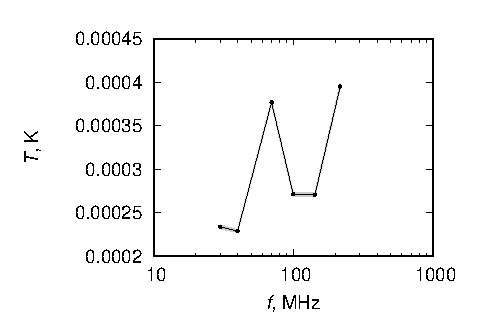
\includegraphics[width=0.5\textwidth]{a_0_wb}} &
			\subfloat[5 arcmin]{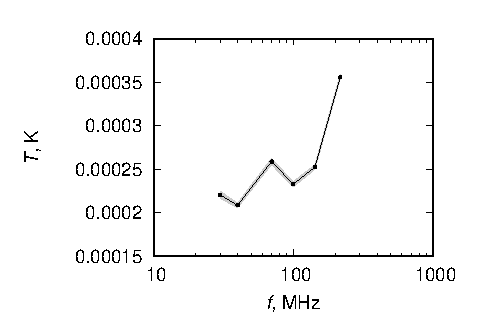
\includegraphics[width=0.5\textwidth]{a_5_wb}} \\
			\subfloat[35 arcmin]{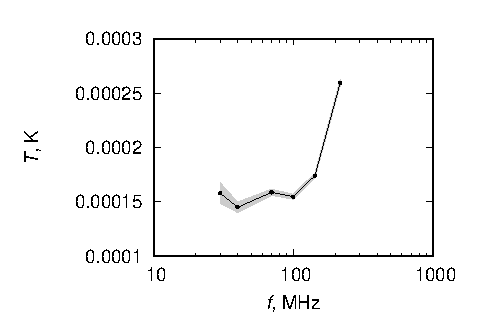
\includegraphics[width=0.5\textwidth]{a_35_wb}} &
			\subfloat[60 arcmin]{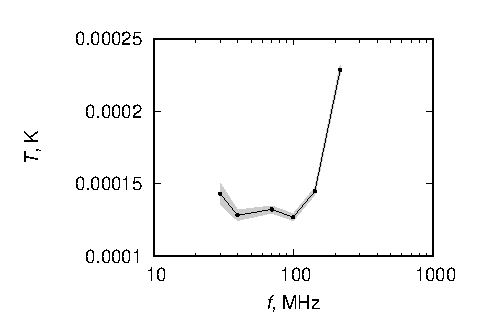
\includegraphics[width=0.5\textwidth]{a_60_wb}} 
		\end{tabular}
		\caption{Усредненный спектр пятен из карты SMICA, построенный по картам различного углового размера сглаживания; по вертикальной оси отложены амплитуды}
		\label{spectrum_amplitude}
	\end{figure}

	\begin{figure}[h!]
		\begin{tabular}{cc}
			\subfloat[0 arcmin]{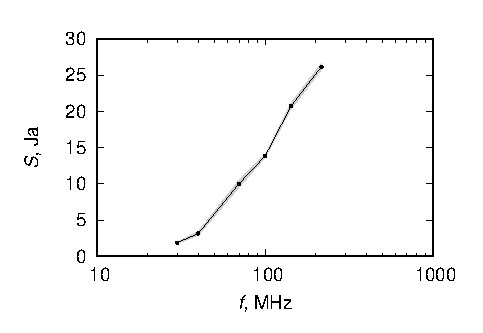
\includegraphics[width=0.5\textwidth]{0_wb}} &
			\subfloat[5 arcmin]{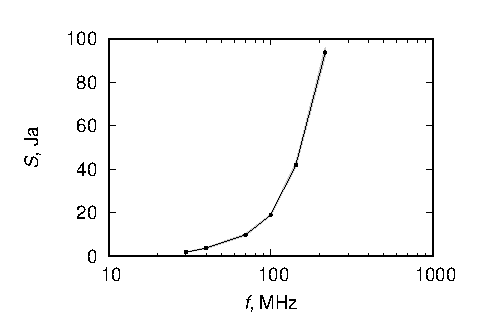
\includegraphics[width=0.5\textwidth]{5_wb}} \\
			\subfloat[35 arcmin]{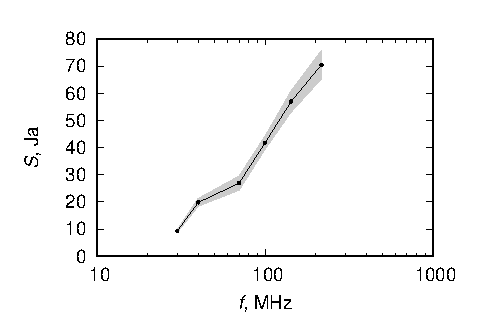
\includegraphics[width=0.5\textwidth]{35_wb}} &
			\subfloat[60 arcmin]{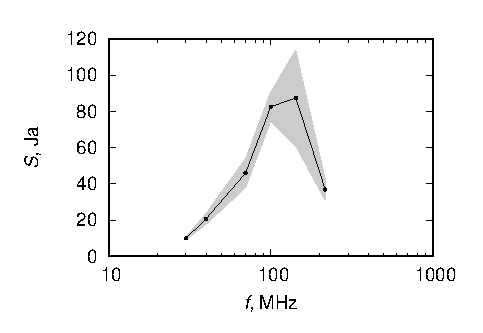
\includegraphics[width=0.5\textwidth]{60_wb}} 
		\end{tabular}
		\caption{Откалиброванный усредненный спектр пятен из карты SMICA, построенный по картам различного углового размера сглаживания; по вертикальной оси отложены плотности потока}
		\label{spectrum_calibrated}
	\end{figure}

\newpage
\section{Выводы}
В результате проделанной работы получено, что замеченный для отдельных пятен микроволнового излучения эффект отклонения спектра от чернотельного типа подтверждается для большой выборки.

\bibliography{report_ref}{}
\bibliographystyle{ugost2008}

\end{document}
